\chapter{Testing}

\section{Overall Approach to Testing}

This chapter presents a multitude of different testing types. There are authomated unit tests to ensure the internal code logic behaves as expected. The User Interface tests are tests which are difficutly to automate but are used to esnure that the user interface encaptures the correct state of execition. Acceptance testing is used to assess how well the applications meets the specified requirements in section \ref{funcymcdunky}. Stress testing has been considered by the author but ultimately has been omitted. The author feels that the application is never subject to heavy loads, nor can the user exceed the normal operational load for the application thus, there is no need to stress test currently.
\section{White-box Testing}
\subsection{Unit Tests}

Unit tests were developed using the JUnit framework and have been designed by the author to test a series of boundary conditions and any underlying algorithmic logic present with the application code. The execution of these tests than then be fully automated and using the built in interface provided by Eclipse a summary of the completed tests can be viewed by the author enabling clear identification of failed tests and reason for failure. The unit tests are generally only performed on the Model package. The view package is difficult to unit test as it requires user input and is therefore manually tested by the author. The controller package does not really contain any behaviour worthy of testing as it mainly consists of simple assignments or the calling of other system functions.

There are features present in the application code which the author has excluded from the unit testing process. Any feature which relies on random numbers to perform its task has not been unit tested. As a random number is used the author feels that they cant reliably be tested, therefore it doesn’t makes sense to attempt to. Instead the author has extracted the code which relies on such random numbers and tested the behaviour of such code using specifically defined values, this enables the author to accurately test for expected behaviours. In addition to this getter and setter methods or simple assignment operations have not been tested. The reason for excluded these methods from unit tests is because the code responsible is so simple it can’t fail so there is no real purpose in producing such tests.

The unit tests that the author has produced revolve around ensuring that only legal algorithm parameters are accepted and that the movement, probability and pheromone functions are behaving as expected and return legal values. These tests contain validation checks against a range of values for each parameter including boundary conditions to ensure that they are correctly dealt with, examples of such testing can be seen in figures \ref{testAlpha} to \ref{testAgent}. The probability and pheromone functions are tested to ensure the correct value is returned and in the case of probability, ensure that the sum of all calculated probabilities is equal to 1, such a test is shown in figure \ref{testProb}. There are many more tests present in the test package for the application however the author has only briefly outlined a small number of these. Evidence of such testing can be seen below in figure \ref{testSS}.

\begin{figure}[H]
\centering
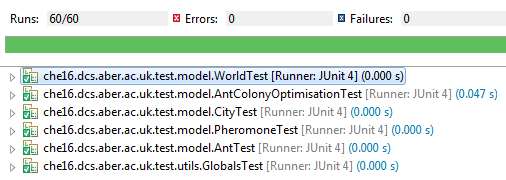
\includegraphics[scale=0.8]{Images/chapter6/testSS}
\caption{Evidence of the completed execution of the applications unit tests. The view present is the built in Eclipse JUnit interface.}
\label{testSS}
\end{figure}

\section{Black-box Testing}
\subsection{User Interface Testing}

It is difficult to reliably test the graphical user interface using a white-boxing testing approach such as the automated unit tests process as mentioned above. To overcome this obstacle the author has decided to manually test the user interface using a black-box testing approach to ensure the correct behaviour to exhibited. The author feels that for the scope and time frame for this project, manually testing the display is the most appropriate form of testing.

During this test process the author did not repeat any form of test that had been previous executed in the unit testing process as these tests are already proved to pass. The tests performed manually by the author will be for the purpose of ensuring that the correct error messages are displayed to the user in the correct situation and making sure the algorithm is being correctly rendered and its current state is modified in as close to real time as possible. 

In addition to testing for errors the file IO process will be tested ensure that configurations can be correctly saved to a specified file and if a user specifies a file to load a configuration from, this file can in fact be handled even if the contents of such file contains incorrect values or bad formatting. Several test files will be produced, each file will be designed to test a variety of possible illegal file contents. Tests will be done to ensure that the application rejects files that contain; missing data, incorrect type for a specified value and City coordinates which exceeds the bounds of the canvas. Files containing such malformed data should not cause the application to crash this will be tested. The saving of a configuration to a file doesn’t not need to be as rigorously tested as the algorithm has to be instantiated with legal values before the writing process can be executed therefore, the values of the written file will be legal and of the correct format. An example of such file contents can be found in appendix D, section \ref{fileIOtest}.

The full list of black-box test performed by the author can be seen in section appendix D, section \ref{BBTests}. The detail and coverage of such tests could be extended however the author feels that for the current state of this project this will suffice.

\subsection{Acceptance Testing}

Due to the lack of a dedicated client acceptance testing proved difficulty for this project. For the purpose of these acceptance tests the author acted as the end user, and used the application in a non-bias manner and adapted the mind-set of a new user. This is far from an ideal way to perform acceptance testing and this process isn’t truly representative of true acceptance tests however, the author felt that for the projects scope it would be sufficient. The application itself is not a finished deployment ready product before this would be the case the author would like to extend current functionality and provide a larger variety of algorithm types and modifiers. If the author had a larger timeframe then a distinct customer or use group would be set up to ensure this acceptance testing process is performed to the highest quality and that the application suits its intended purpose. The results of this process can be found in appendix D, \ref{BBTests}.
